\documentclass{ifacconf}

% Warning: different journals/conferences migh have different requirements for the papers this is just a default template

%*********************************************************************************************************************************

% Importing packages -  beginning


%\usepackage{cite}
\usepackage{amssymb,amsfonts}
\usepackage{amsmath}
\interdisplaylinepenalty=2500
\usepackage{algorithmic}
\usepackage{graphicx}
\usepackage{textcomp}
\usepackage{xcolor}
\def\BibTeX{{\rm B\kern-.05em{\sc i\kern-.025em b}\kern-.08em
		T\kern-.1667em\lower.7ex\hbox{E}\kern-.125emX}}	


\makeatletter
\def\endthebibliography{
	\def\@noitemerr{\@latex@warning{Empty `thebibliography' environment}}
	\endlist
}
\makeatother

\renewcommand{\encodingdefault}{OT1}
\usepackage[utf8]{luainputenc}
\usepackage[withpage, nohyperlinks]{acronym}
\usepackage[spaces,hyphens]{xurl}
\usepackage{caption}
\usepackage{glossaries-extra}
%\usepackage{natbib} 
\usepackage[round,sort,comma,numbers]{natbib}


% Importing packages - end

% Solving problem with hyperref package when used with IFAC template - beginning

% At first you have to compile the finished document with the package hyperlink commented out and then
% uncomment the package import otherwise the file might not be compiled properly

%\usepackage[colorlinks,allcolors=blue]{hyperref}

% Solving problem with hyperref package when used with IFAC template - end

%*********************************************************************************************************************************


\begin{document}
	\urlstyle{tt}
	
	\begin{frontmatter}
	
		% Paper titles should be written in uppercase and lowercase letters, not all uppercase.
		\title{Template for IFAC Papers \thanksref{footnoteinfo}}
		
		\thanks[footnoteinfo]{Sponsor and financial support acknowledgment
			goes here.}
	
		\author[First]{Batman} 
\author[First]{Homer Simpson} 
\author[First]{Joker}

\address[First]{Department of Technical Cybernetics,\\
				Faculty of Management Science and Informatics,\\ 
				University of Žilina, \\
				Slovakia, Žilina \\ 
				(e-mail:
				batman@fri.uniza.sk, 
				homer.simpson@fri.uniza.sk, 
				joker@fri.uniza.sk   
				)}



%\author[First]{First A. Author} 
%\author[Second]{Second B. Author, Jr.} 
%\author[Third]{Third C. Author}
%
%\address[First]{National Institute of Standards and Technology, 
%	Boulder, CO 80305 USA (e-mail: author@ boulder.nist.gov).}
%\address[Second]{Colorado State University, 
%	Fort Collins, CO 80523 USA (e-mail: author@lamar. colostate.edu)}
%\address[Third]{Electrical Engineering Department, 
%	Seoul National University, Seoul, Korea, (e-mail: author@snu.ac.kr)}
	
		\begin{abstract}
	Here you write abstract.
\end{abstract}

\begin{keyword}
	Here you write key words.
\end{keyword}
	
	\end{frontmatter}
	
	%Glossary
	\section*{List of Acronyms}

% With the following command we can add padding between acronym and its meaning
\renewcommand{\IEEEiedlistdecl}{\IEEEsetlabelwidth{SONET}}

\begin{acronym}
	\hypersetup{hidelinks}
	
	\acro{ram}[RAM]{Random Access Memory}
	\acro{fri}[FRI]{Faculty of Management Science and Informatics}
	\acro{iot}[IoT]{Internet-of-Things}
	
	\acrodefplural{iot}[IoTs]{Internets-of-Things}
	
\end{acronym}

\renewcommand{\IEEEiedlistdecl}{\relax} %reset back
	
		
	\section{INTRODUCTION}

This is the introduction of the paper.
	
	% Add here the sections of your conference paper - beginning
	
	\section{MY ONLY SECTION}


Conference papers use normal size for the first letter of the conference paper.

The \ac{iot} is becoming very popular. One of the elements of \ac{iot} are embedded systems. There is a lot of \aclp{iot} devices currently on the market the acronym for them is \acsp{iot}.

On the \acf{fri} you will learn about \acs{ram} which is short for \acl{ram}.

The monkeys are very smart animals \cite{article_first}. They are shown in \figurename ~\ref{fig:monkey}. 

\begin{figure}[ht]
	\centering
	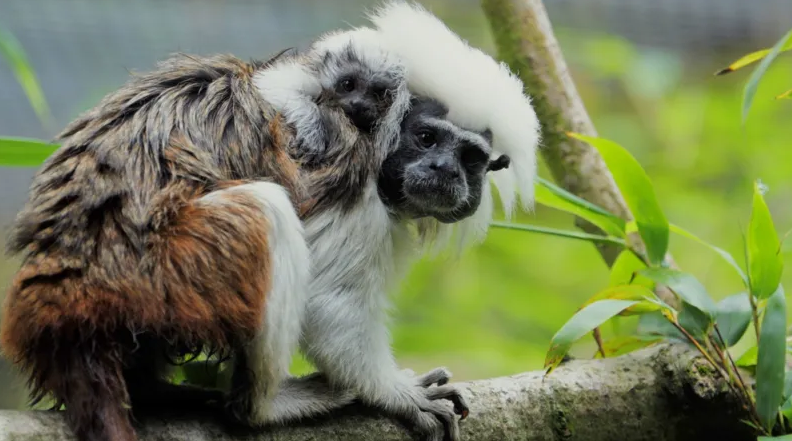
\includegraphics[width=1.0\linewidth]{pictures/monkey}
	\caption{Nice picture of monkey \cite{figure_first}}
	\label{fig:monkey}
\end{figure}


We can use vibrational energy harvesting during monkey studies \cite{article_second}. Its basic principle is shown in \figurename  ~\ref{fig:vibrationalenergyharvesting}.

\begin{figure}[ht]
	\centering
	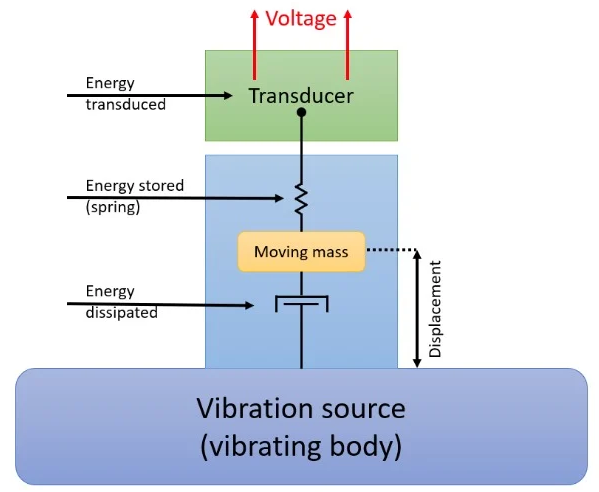
\includegraphics[width=1.0\linewidth]{pictures/vibrational_energy_harvesting}
	\caption{Vibrational energy harvesting principle \cite{figure_second}}
	\label{fig:vibrationalenergyharvesting}
\end{figure}

This is how you should cite text that has multiple sources \cite{article_first, article_second}.

In table \ref{tab:first_table} we have some measured data.

\begin{table}[ht]
	\centering
	\caption{My first table}
	\label{tab:first_table}
	\begin{tabular}{|c|c|c|c|}
		\hline
		& $a$ & $b$ & $c$ \\
		\hline
		$a$ & 1 & 0 & 1 \\
		\hline
		$b$ & 0 & 1 & 1 \\
		\hline
		$c$ & 1 & 1 & 0 \\
		\hline
	\end{tabular}
\end{table}

And in the \eqref{eq:original_equation} is shown a very simple formula. Based on which the variable $a$ is a sum of two variables $b$ and $c$.

\begin{equation}
	\label{eq:original_equation}
	a = b + c
\end{equation}

We can also calculate the value of variable $c$ by altering the equation as in \eqref{eq:altered_equation}. 

\begin{equation}
	\label{eq:altered_equation}
	c = a - b
\end{equation}

This way we can create a plain unnumbered list.

\begin{list}{}{}
	\item Hope
	\item Elizabeth
	\item Josette 
\end{list}

This way we can create an unnumbered list.

\begin{itemize}
	\item Hope
	\item Elizabeth
	\item Josette
\end{itemize}

This way we can create an numbered list.

\begin{enumerate} 
	\item Hope
	\item Elizabeth
	\item Josette
\end{enumerate}

This way we can create lists with descriptions.

\begin{description}
	\item[red] nice colour
	\item[blue] not very nice colour
\end{description}
	
	
	% Add here the sections of your conference paper - end
	
	
	\section{CONCLUSION}

This is the conclusion of the paper.

	
	
	
	\section*{Declaration of Competing Interests}

The authors declare that they have no known competing financial interest or personal relationships that could have appeared to influence the work reported in this paper.
	
	\section*{Data availability}

No data was used for the research described in the article.
	
	
	\section*{Acknowledgment}

This work was supported by the National Foundation of Quantum Telecommunications (Grant No. 123456789).
	
	
	
	% If you are using TexStudiu you have to choose Tools → Commands → Bibtex and then recompile to sort the references based on their order of citations in the document.
	% You can also add shortcut for Bibtex to the upper menu. Based on pictures from the folder bibliography_recompilation_guide. 
	
	% If you are using Overleaf then it will automatically sort the references for you.
	\nocite{*}
	\bibliography{./bibliography/figure_sources.bib,./bibliography/text_sources.bib}
	%\bibliography{./bibliography/refs-test-delete.bib}
	
	
	\appendix
	\section{A summary of Latin grammar}    % Each appendix must have a short title.
	\section{Some Latin vocabulary}         % Sections and subsections are supported  
	
	
\end{document}

\begin{comment}
	
% If you don't know what to put to certain fields don't erase them just leave them empty they will be automatically ignored when the references are generated.

% Template for articles in biblography

@article{,
	title        = {},
	author       = {},
	year         = {},
	month        = {},
	journal      = {},
	booktitle    = {},
	volume       = {},
	number       = {},
	pages        = {},
	doi          = {},
	issn         = {},
	url          = {},
}

% Example usage 

@article{vibrations,
	title        = {A study of low level vibrations as a power source for wireless sensor nodes},
	author       = {Shad Roundy and Paul K. Wright and Jan Rabaey},
	year         = {2003},
	month        = {July},
	journal      = {Computer Communications},
	booktitle    = {},
	volume       = {26},
	number       = {11},
	pages        = {1131--1144},
	doi          = {https://doi.org/10.1016/S0140-3664(02)00248-7},
	issn         = {0140-3664},
	url          = {https://www.sciencedirect.com/science/article/pii/S0140366402002487},
}

% Template for Figures in biblography

% Template for Figures in biblography

@online{,
	title        = {},
	author       = {},
	year         = {},
	month		 = {},
	publisher 	 = {},
	urldate   	 = {},
	url          = {},
}


% Example usage

@online{vibrations,
	title        = {Introduction to Vibration Energy Harvesting},
	author       = {Francesco Orfei},
	year         = {2019},
	month		 = {June},
	publisher 	 = {allaboutcircuits},
	urldate   	 = {10.9.2023},
	url          = {https://www.allaboutcircuits.com/technical-articles/introduction-to-vibration-energy-harvesting/},
}

\end{comment}
